\chapter{Analog amplifiers}

\section{Common Emitter Amplifier}
The

\begin{figure}[H]
    \centering
    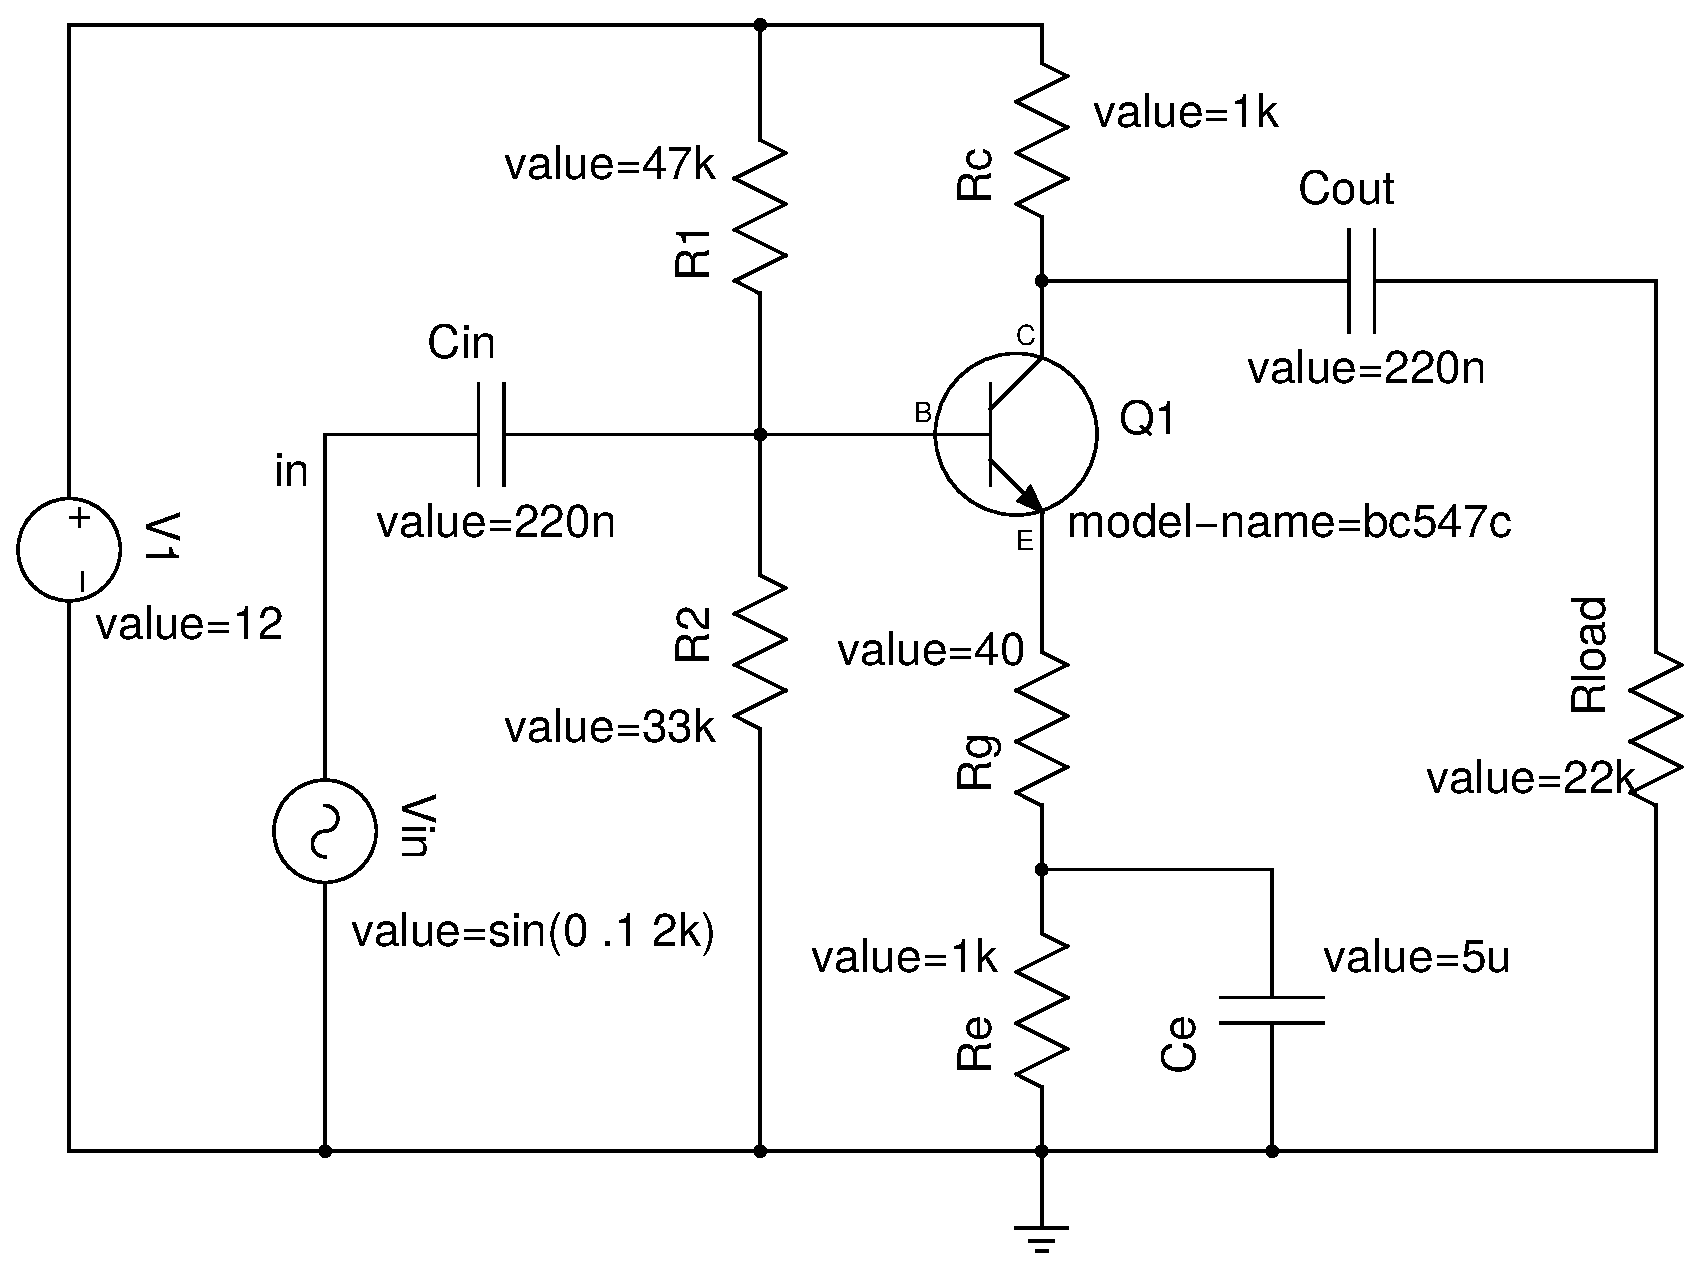
\includegraphics[scale=0.45]{ce-amplifier}\label{ce-amplifier}
    \caption{Circuit diagram for the common emitter amplifier}
\end{figure}

The

\section{ngSPICE}
Simulation output.

\begin{figure}[H]
    \centering
    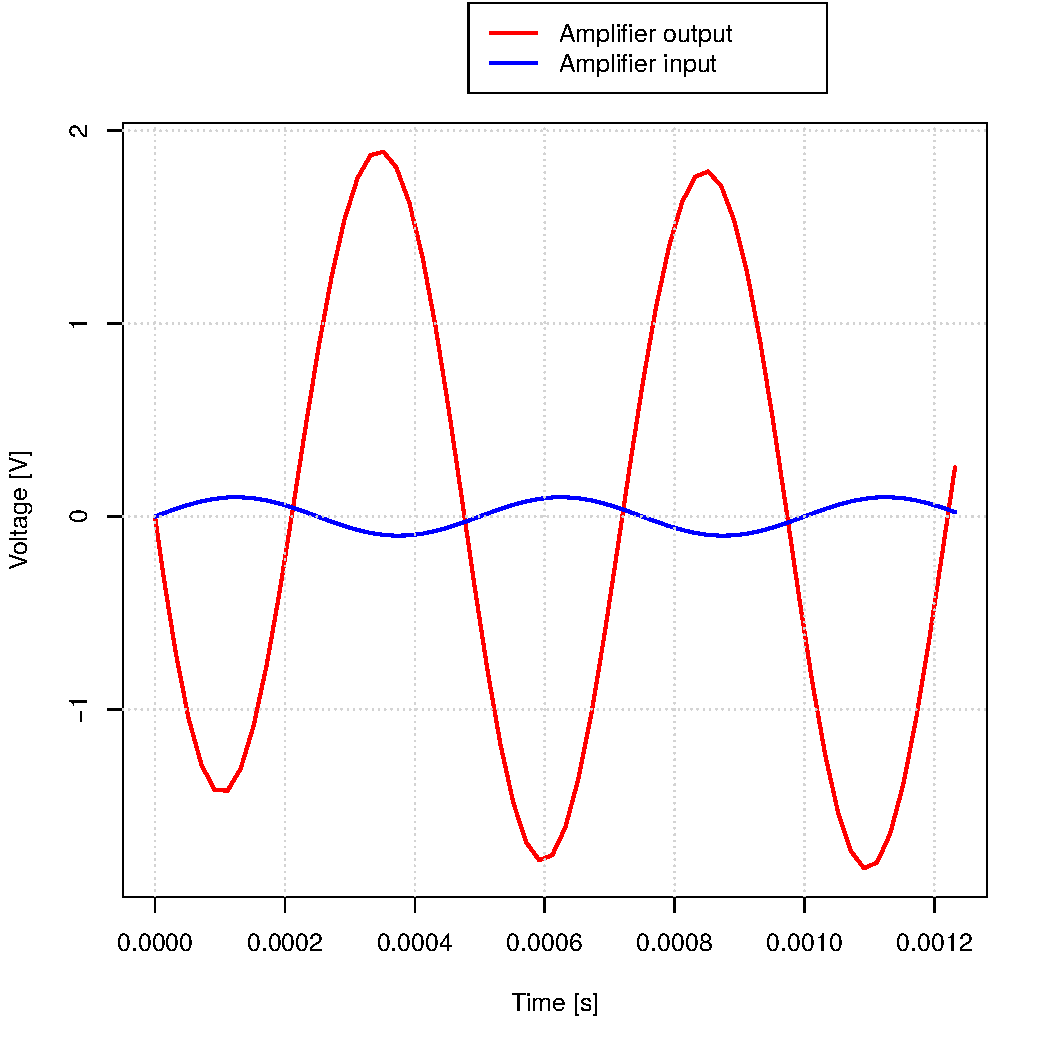
\includegraphics[scale=.7]{ce-amplifier-sim}\label{ce-amplifier-sim}
    \caption{Simulation of the common emitter amplifier}
\end{figure}

\begin{lstlisting}
 amplifier
.model bc547c NPN (BF=730 NE=1.4 ISE=29.5F IKF=80M IS=60F VAF=25 ikr=12m
       + BR=10 NC=2 VAR=10 RB=280 RE=1 RC=40 VJE=.48 tr=.3u tf=.5n
       + cje=12p vje=.48 mje=.5 cjc=6p vjc=.7 mjc=.33 isc=47.6p kf=2f)
Vin in 0 sin(0 .1 2k)
V1 4 0 9
Ce 0 5 5u
Cout 1 out 220n
Cin in 3 220n
Rc 1 4 1k
Rload 0 out 22k
Re 0 5 1k
Rg 5 2 40
R2 0 3 33k
R1 3 4 47k
Q1 1 3 2 bc547c
.TRAN 15u 1.23m
.end
\end{lstlisting}

Represented by.